\chapter{Getting help}

\section{The man command}

A manual (man) page is  a text-based help file for a specific command, service, or configuration file. These pages are stored in 	\verb|/usr/man| or \verb|/usr/share/man|. The \verb|MANPATH| environment variable is used to identify location of man pages. Each man page contains information about a specific type of files or commands, which have become the \emph{sections} listed below:

\begin{enumerate}
\item User commands (both executable and shell programs)
\item System calls
\item Library functions
\item Special files (such as device files)
\item File formats (configuration files and structures)
\item Games
\item Conventions, standards, miscellaneous (protocols, file systems)
\item System administration and privileged commands
\item Linux kernel API
\end{enumerate}

To distinguish identical topic names in different sections, man page references include the section number in parentheses after the topic. For example, \verb|passwd(1)| describes the command to change passwords, while \verb|passwd(5)| explains the \verb|/etc/passwd| file format for storing local user accounts.\\

To read specific man pages, user \code{man <topic>} command. For example, \verb|man passwd| displays man pages about \verb|passwd| command. To display the man page topic from a specific section, please include the section number argument, for example, \verb|man 5 passwd| displays \verb|passwd(5)| man pages. The command \verb|man -k <string>| performs a keyword search, which displays a list of keyword-matching man pages with section numbers.

\begin{table}[hbtp]
\centering\caption{Navigating man pages}
\begin{tabular}{|l| p{10cm} |}
\hline 
\head{Command}&\head{Result}\\
\hline 

\verb|Spacebar|, \verb|PgDown| & Scroll down one screen\\
\hline 
\verb|PgUp|, \verb|b| & Scroll up one screen\\
\hline 
\verb|d| & Scroll down one half-screen\\
\hline 
\verb|u| & Scroll up one half-screen\\
\hline 
Up/Down arrow & Scroll up/down one line\\
\hline 
\verb|/string|& Search forward for \verb|string|\\
\hline 
\verb|n|& Repeat the previous search forward\\
\hline 
\verb|N|& Repeat the previous search backward\\
\hline  
\verb|g|& Go to the start of the man page\\
\hline 
\verb|G|& Go to the end of the man page\\
\hline 
\verb|q|& Exit man page and return to the command shell prompt\\
\hline 
\end{tabular}
\end{table}

Each man page is broken into sections. Each section is designed to provide specific information about a command. The table \ref{tab:SecMan} describes some of the more common sections that you will find in man pages.

\begin{table}[hbtp]
\centering\caption{Sections in each man page}\label{tab:SecMan}
\begin{tabular}{|l| p{13cm} |}
\hline 
\head{Section}&\head{Purpose}\\
\hline 
NAME & Provides the name of the command and a very brief description.\\ \hline 
SYNOPSIS & A brief summary of the command or function's interface. A summary of how the command line syntax of the program looks.\\
DESCRIPTION & Provides a more detailed description of the command.\\ \hline 
OPTIONS & Lists the options for the command as well as a description of how they are used. Often this information will be found in the DESCRIPTION section and not in a separate OPTIONS section.\\ \hline 
FILES & Lists the files that are associated with the command as well as a description of how they are used. These files may be used to configure the command's more advanced features. Often this information will be found in the DESCRIPTION section and not in a separate FILES section.\\ \hline 
AUTHOR & The name of the person who created the man page and (sometimes) how to contact the person.\\ \hline 
REPORTING BUGS & Provides details on how to report problems with the command. \\ \hline 
COPYRIGHT & Provides basic copyright information.\\ \hline 
SEE ALSO & Provides you with an idea of where you can find additional information. This also will often include other commands that are related to this command.\\ \hline 
\end{tabular}
\end{table}

The \verb|-t| option of \verb|man| command prepares a man page for printing in PostScript format (\verb|.ps| extension). To view this PostScript file, use \verb|evince| command:

\begin{verbatim}
$ man -t passwd > passwd.ps
$ evince passwd.ps
$ evince -w passwd.ps
$ evince -i 3  passwd.ps
$ lp passwd.ps -P -2 -3
\end{verbatim}

While the normal \verb|evince| mode allows full-screen viewing, the preview mode (\verb|-w| option) provides quick browsing and printing preview. The \verb|-i| option is used to specify the starting page. The \verb|lp| command sends page 2 and 3 of this PostScript file to the default printer for real printing.

\section{The pinfo command}

GNU Project developed a different online documentation system, known as GNU info. Info documentations are structured as hyperlinked info nodes and more in-depth than man pages. Info nodes for a particular topic are browsed with the \verb|pinfo <topic>| command (Table \ref{tab:NaviInfo}).\\

\begin{table}[hbtp]
\centering\caption{Navigating info pages}\label{tab:NaviInfo}
\begin{tabular}{|p{3cm}| p{10cm} |}
\hline 
\head{Command}&\head{Result}\\
\hline 

\verb|Spacebar|, \verb|PgDown| & Scroll down one screen\\
\hline 
\verb|PgUp|, \verb|b| & Scroll up one screen\\
\hline 
\verb|d| & Display the directory of the topics\\
\hline 
\verb|u| & Display the parent node\\
\hline 
\verb|HOME| & Display the top of a topic\\
\hline 
Up/Down arrow & Scroll up/down one hyperlink\\
\hline 
\verb|ENTER|& Open topic at cursor location\\
\hline 
\verb|/string|& Search forward for \verb|string|\\
\hline 
\verb|n|& Display the next node in the topic\\
\hline 
\verb|/| then \verb|ENTER|& Repeat the previous search forward\\
\hline
\verb|p|& Display the previous node in the topic\\
\hline 
\verb|q|& Exit man page and return to the command shell prompt\\
\hline 
\end{tabular}
\end{table}

\section{Reading documentation in /usr/share/doc}

Bundling documentation with RPM packages are stored in the directory \verb|/usr/share/doc/|. When the package is installed, files recognized as documentation are moved to \verb|\usr/share/doc/<pkg-name>|. Use \verb|less| or \verb|gedit| to read text-based file. Use a browser to read a PDF- or HTML-based documentation.

\begin{verbatim}
[student@serverX doc]$ less vim-common-*/README.txt
[student@serverX doc]$ firefox grub2-common-2.02/grub.html
\end{verbatim}

Some software provides its document as a separate package. For example, the \verb|gnuplot| program has the extra \verb|gnuplot-doc| package, which must be installed separately. Use \verb|yum| to display only those packages that contain \verb|-doc|, or \verb|documentation|.\\

\note The \verb|kernel-doc| package has kernel, driver, tuning, and advanced configuration information.

\section{Use redhat-support-tool}

\subsection{Introduction}

Red Hat provides a text console interface to the subscription-based Red Hat Customer Portal. Internet access is required to have access to this service. This tool is text-based for use from any terminal or SSH connection; no graphical interface is provided. The \verb|redhat-support-tool| command can be used as either interactive shell (by default) or invoked as individually executed commands. When first invoked, this tool requires Red Hat Access subscriber login information. To avoid repetitively supplying this account information, a user can store it in his/her home directory:

\begin{verbatim}
~/.redhat-support-tool/redhat-support-tool.conf
\end{verbatim}

If a Red Hat account is shared by many people, the \verb|--global| option can save account information to \verb|/etc/| directory:

\begin{verbatim}
/etc/redhat-support-tool.conf
\end{verbatim}

\subsection{Red Hat Knowledgebase}

The \verb|redhat-support-tool| command allows subscribers to search and display the same Knowledgebase content seen when on the Red Hat Customer Portal. The Knowledgebase permits keyword searches (similar to to the \verb|man| command). Users can enter error codes, syntax from log files, or any mix of keywords to produce a list of relevant solution documents.

\begin{figure}[hbtp]
\caption{Keyword search feature }
\centering
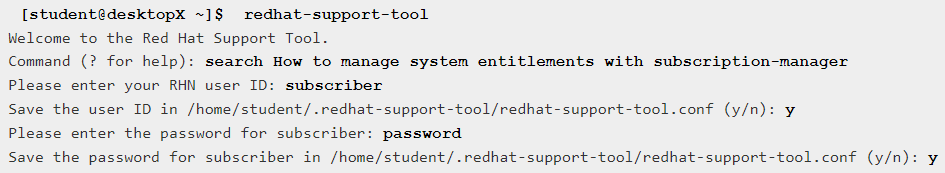
\includegraphics[ scale=0.5 ]{pictures/BasicRHtool.PNG}
\end{figure}

Red Hat subscribers can also locate online articles using Knowledgebase document ID:

\begin{verbatim}
$ redhat-support-tool kb 253273 | less
\end{verbatim}

\subsection{Bug report}

Another benefit of the \verb|redhat-support-tool| command is that users can gather relevant information for a bug report. In the bug report, the problem and its symptoms must be clarified. Background information (which product is affected, version, etc.) is also required. For kernel problems, Red Hat uses kernel crash dump core files to create and extract \emph{backtrace}\footnote{a report of active stack frames at the point of the crash} to provide onsite diagnostic and open a support case. Therefore, system's \textbf{kdump} crash dump or a digital photo of the kernel backtrace display must be included in the SoS report.\\

Red Hat uses four severity levels to classify issues. The \textbf{Urgent} and \textbf{High} severity problem reports should be followed by a phone cal to the relevant local support center.\\

\begin{enumerate}
\item \textbf{Urgent:} A problem that severely impacts your use of the software in a production environment (e.g. loss of data, production systems are not functioning). The situation \emph{halts} your business operations and \emph{no procedural} workaround exists.

\item \textbf{High:} A problem where the software is \emph{functioning} but your use in a production environment is \emph{severely reduced}. The situation is causing a \emph{high impact} to portions of your business operations and \emph{no procedural} workaround exists.

\item \textbf{Medium:} A problem that involves \emph{partial}, \emph{non-critical} loss of use of the software. For production environments, there is a \emph{medium-to-low} impact on your business, but your business \emph{continues to function}, including a procedural workaround. For development environments, your business \emph{migrates into production} or \emph{no longer to continue}.

\item \textbf{Low:} A general usage question, reporting of a documentation error, or recommendation for a future product enhancement or modification. For production environments, there is a low-to-no impact on your business. For development environments, there is a medium-to-low impact but your business continues to function.
\end{enumerate}

When support cases are opened, users may create a diagnostic reports using \verb|sosreport| sub-command of \verb|redhat-support-tool|. This command stores the report in \verb|/var/tmp/| directory as an \verb|xz| archive. 

\begin{verbatim}
# sosreport
# cd /var/tmp/
# tar -xvJf sosreport-*.tar.xz
# cd sosreport-yourname.01034221-0164831865
\end{verbatim}

Users can also upload and attache files to online cases. Case detail including \emph{product}, \emph{version}, \emph{summary}, \emph{description}, \emph{severity}, and \emph{case group}. In the picture \ref{OpenCase}, the \verb|--product| and \verb|--version| are specified using \verb|opencase| command.\\

\begin{figure}[hbtp]
\caption{Open a case}\label{OpenCase}
\centering
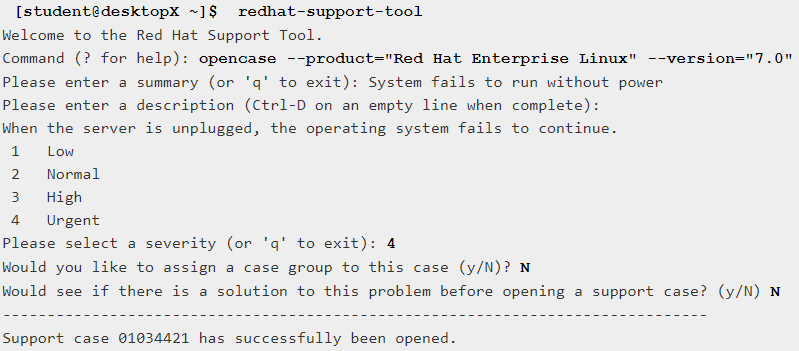
\includegraphics[ scale=0.5 ]{pictures/OpenCase.PNG}
\end{figure}

Including diagnostic information when a support case is first created contributes to quicker problem resolution. The \verb|sosreport| command generates a compressed tar archive of diagnostic information gathered from the running system. If a current SoS report is not already prepared, an admin can generate and attach one later, using the \verb|addattachment| command. Support cases can also be modified by the subscribers (picture \ref{ListCase}).\\

\begin{figure}[hbtp]
\caption{View, Modify a case}\label{ListCase}
\centering
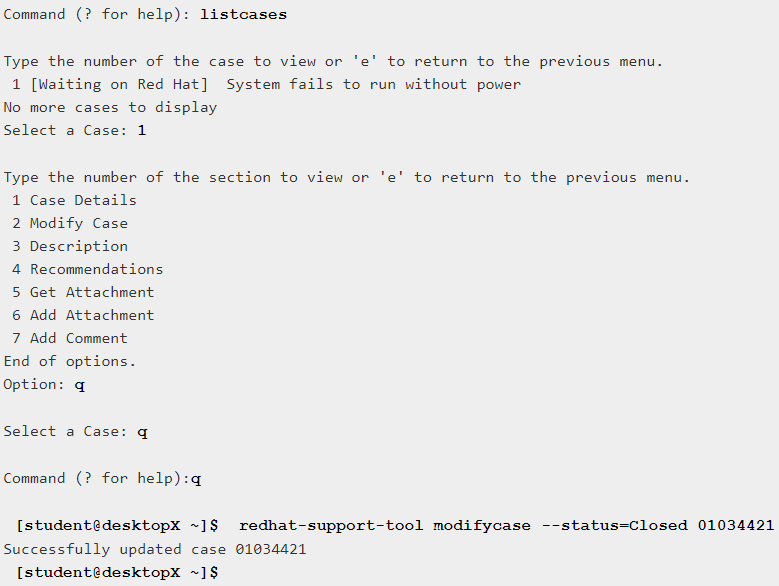
\includegraphics[scale=0.5]{pictures/ListCase.PNG}
\end{figure}

The \verb|redhat-support-tool| also support log file analysis. The tool's \verb|analyze| command log files of many types. The analysis result can be parsed to recognize problem symptoms. 

